%!TEX root = ../bachelorthesis.tex
\chapter{Architektur}
\label{chap:architektur}
Für dieses Projekt wurden mehrere Softwareprogramme integriert, teilweise wurden eigene Programme geschrieben. In den folgenden Abschnitten wird ein Gesamtüberblick gegeben und die einzelnen Programme werden hinsichtlich ihrer Aufgaben detailliert beschrieben.

\section{Gesamtübersicht} % (fold)
\label{sec:gesamtübersicht}
In \autoref{img:overview} ist die Architektur graphisch dargestellt. Jeder Knoten stellt dabei eine ROS-Node dar, also ein einzelnes Programm. Knoten, die blau eingefärbt sind, stehen für Programme, die von anderen Benutzern programmiert wurden und gegebenenfalls zu diesem Einsatzzweck angepasst wurden. Programme, die im Rahmen dieser Bachelorarbeit programmiert wurden, sind grün eingefärbt.
\begin{figure}[!hbt]
	\centering
	\vspace{1ex}
	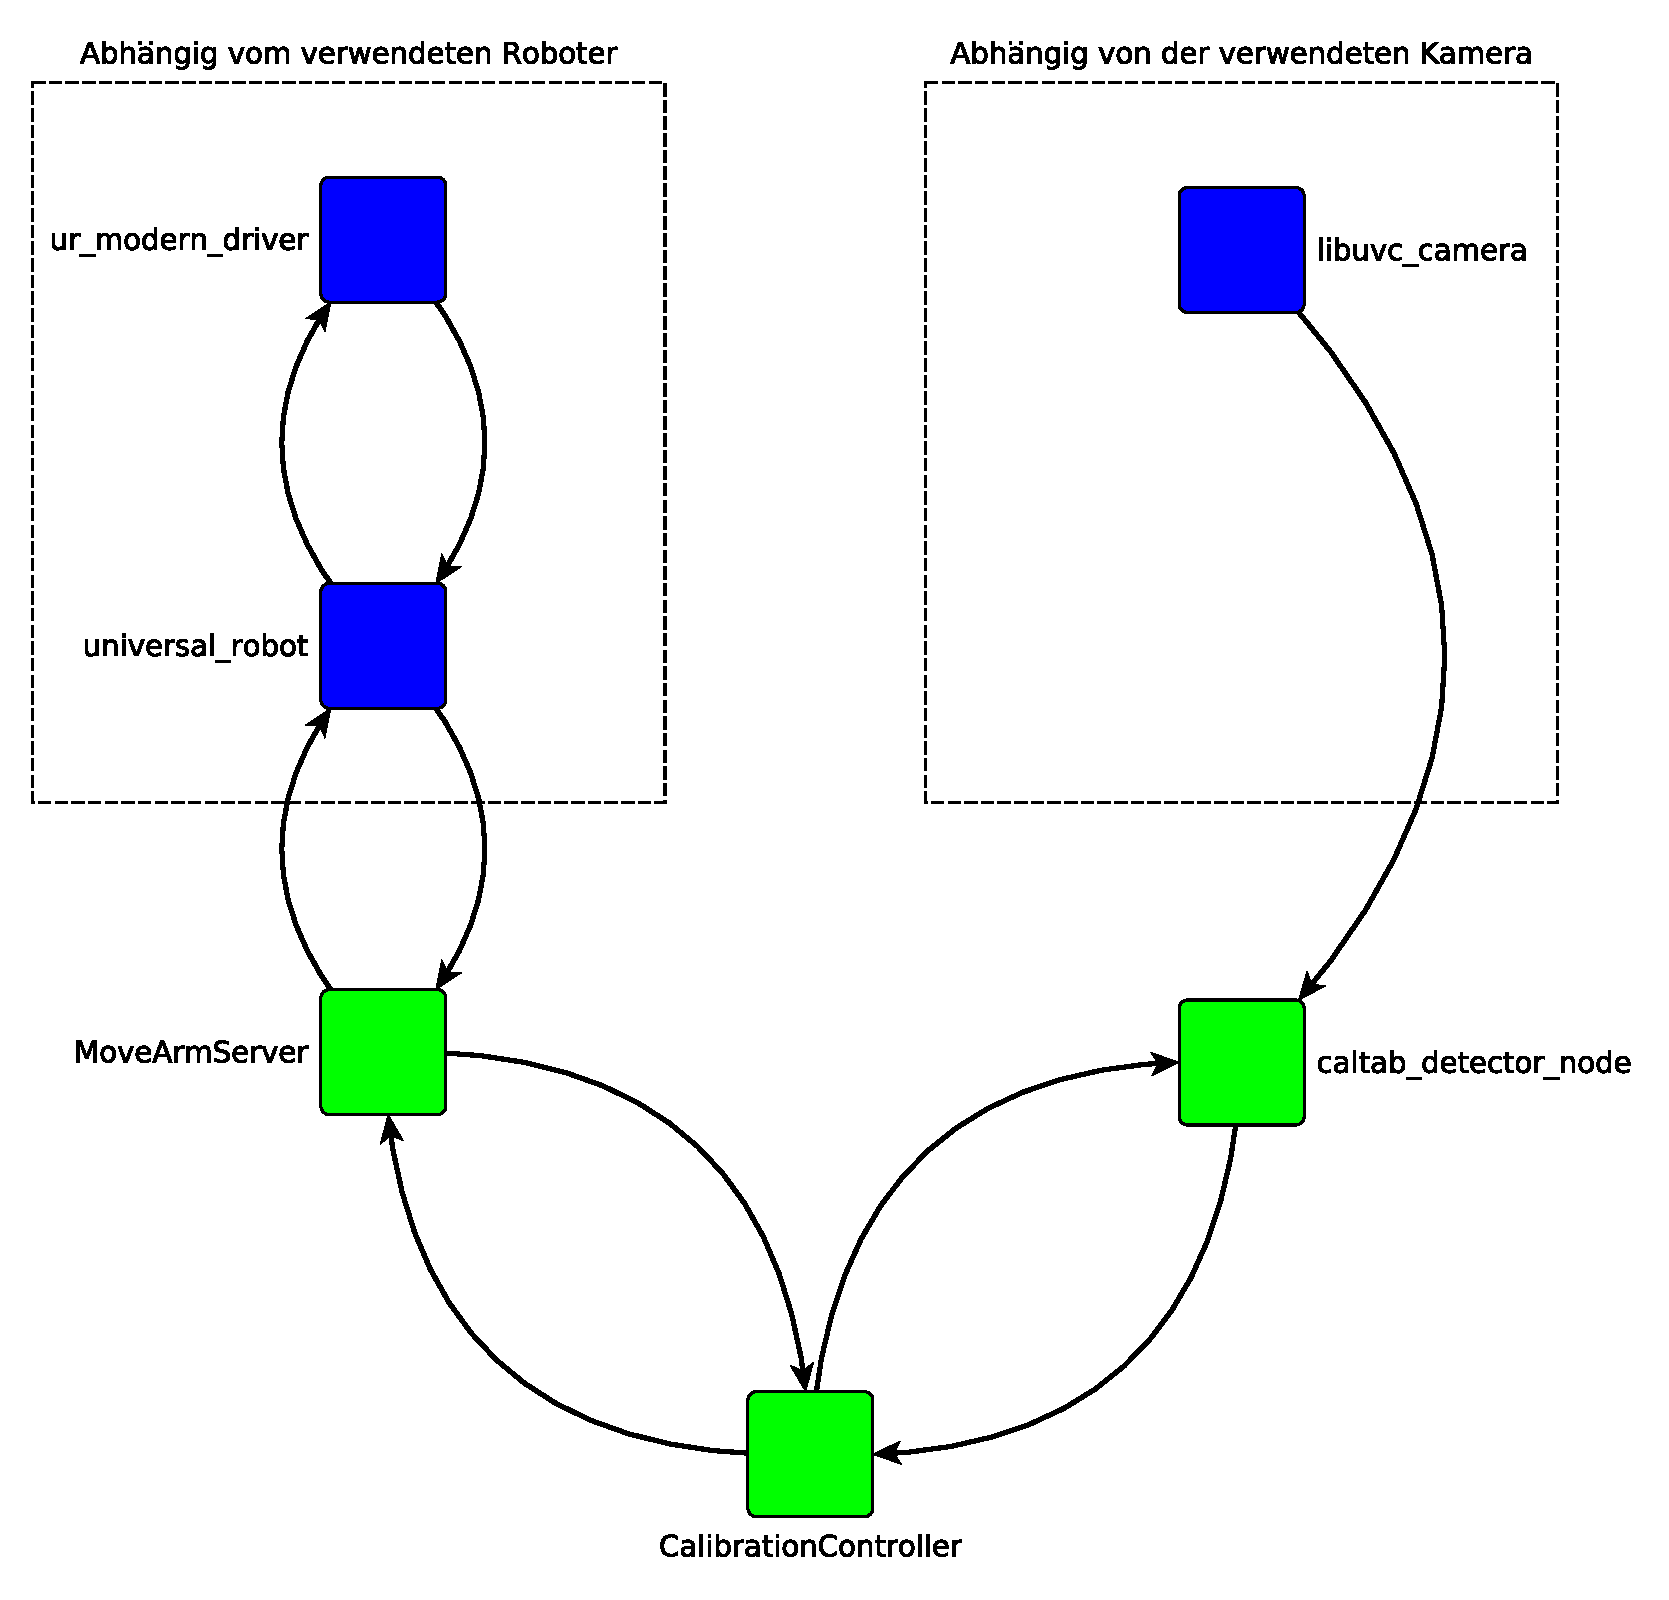
\includegraphics[scale=0.6]{../images/overview}
	\caption[Übersicht über die Architektur. Die Pfeile verdeutlichen die Kommunikation zwischen den Knoten.]{\label{img:overview} Übersicht über die Architektur}
	\vspace{1ex}
\end{figure}
\todo{Übersetzung von Architekturnamen zu tatsächlichen Klassennamen fehlt.}
Die Robot Hardware Interface Node stellt eine Schnittstelle bereit, damit ROS-Pakete wie MoveIt! den Roboter steuern können.

Die Moveit Path Planning Node startet MoveIt! und die dazugehörigen Programme, um MoveIt! zum Planen und Ausführen von Bewegungen nutzen zu können.

Die Camera Interface Node veröffentlicht das Kamerabild über einen ROS Topic.

Die Client Side Path Planning Node stellt eine weitere Abstraktionsschicht zur Bewegung des Arms zur Verfügung. Sie bereitet die Positionsziele für MoveIt! auf und startet die Auswertung von Bildern.

Die Computer Vision Node wertet die empfangenen Bilder der Kamera aus.

Die Highlevel Executive Node steuert den gesamten Ablauf.

\section{Robot Hardware Interface Node} % (fold)
\label{sec:ur_modern_driver}
Für diese Node wird das Paket \texttt{ur\_modern\_driver} verwendet, siehe \cite{ur_modern_driver}. Sie ist die Schnittstelle zwischen dem Roboterarm UR5 und dem ROS Framework. Da dieses Paket nicht für die in diesem Projekt benutzte Version von ROS entwickelt wurde, wurden einige wenige Anpassungen am Sourcecode vorgenommen, um das es in diesem Projekt benutzen zu können.

\section{Moveit Path Planning Node} % (fold)
\label{sec:universal_robot}
Auch für diese Node wird ein öffentlich verfügbares Paket genommen: \texttt{universal\_robot}, siehe \cite{universal_robot}. In dieser Node ist MoveIt! integriert, welches zum Bewegen des Roboterarms benutzt wird. Siehe \autoref{ssub:moveit} für weitere Details über MoveIt!.

\section{Camera Interface Node} % (fold)
\label{sec:libuvc_camera}
Auch diese Node ist als Paket \texttt{libuvc\_camera} in ROS verfügbar. Sie dient dazu, das Bild der angeschlossenen Webcam über ROS verfügbar zu machen. In dem Script, mit dem diese Node gestartet wird, lassen sich verschiedene Parameter einstellen. In diesem Fall wurde mittels der Vendor-ID und Product-ID die zu benutzende Kamera definiert, die Auflösung wurde auf Full-HD gesetzt und der Fokus wurde so eingestellt, dass der Bereich, in dem sich das Kalibrierungsmuster befinden wird, scharf zu sehen ist.

\section{Client Side Path Planning Node} % (fold)
\label{sec:movearmserver}
Dieses Programm wurde im Rahmen dieser Bachelorarbeit selbst entwickelt. Es dient dazu, der Highlevel Executive Node eine weitere Abstraktionsschicht zum Bewegen des Arms zu bieten.

Dazu wurde ein Actionserver erstellt, der die Position des Kalibrierungsmusters als Auftrag erhält. Zusätzlich kann als weiterer Parameter für den Auftrag die Neigung des Musters angegeben werden. Das Programm berechnet dann für die gewünschte Position zunächst die Orientierung für den Roboterendpunkt, damit das Muster senkrecht zur Kamera steht. Anschließend wird zu der berechneten Orientierung die gewünschte Neigung hinzugefügt. Die so errechnete Position und Orientierung wird dann an MoveIt! übergeben. Abhängig davon, ob MoveIt! den Arm erfolgreich bewegen konnte, informiert diese Node den Highlevel Executive Controller, ob der Auftrag erfolgreich ausgeführt wurde.

\section{Computer Vision Node} % (fold)
\label{sec:caltab_detector_node}
Auch dieses Programm wurde selbst entwickelt. Es benutzt die Bibliothek von HALCON, um in den Bildern, die es von der Kamera empfängt, nach dem Kalibrierungsmuster zu suchen und die Kalibrierung durchzuführen.

Diese Node bietet zwei Actionserver an. Der erste Actionserver erwartet einen Auftrag, um in den aktuellen Bildern nach dem Kalibrierungsmuster zu suchen. Dazu wird ein Parameter übergeben, der angibt, wie viele Bilder ausgewertet werden sollen. Die Algorithmen von HALCON finden nicht immer im ersten Versuch das Muster, daher lässt sich die Anzahl der Bilder mit Hilfe dieses Parameters definieren. Die Node meldet dem Highlevel Executive Controller zurück, ob nach der angegeben Anzahl der Bilder das Muster gefunden wurde oder nicht.

Der zweite Actionserver nimmt den Auftrag zur Durchführung der Kalibrierung an. Dazu werden die Bilder, in denen das Muster zu sehen war, ausgewertet. Danach werden die errechneten intrinsischen Parameter, die Verzeichnungsparameter sowie der ermittelte durchschnittliche Fehler an den Highlevel Executive Controller zurückgegeben.

\section{Highlevel Executive Controller} % (fold)
\label{sec:calibrationcontroller}
Diese letzte Node wurde ebenfalls selbst entwickelt. Sie dient dazu, den gesamten Ablauf der Kalibrierung zu steuern, indem sie die Actionserver mit Aufgaben versorgt. Zunächst übergibt der Benutzer dem Programm die Position der Kamera in Relation zur Basis des Roboterarms und die initialen intrinsischen Parameter. Dann wird aus diesen Werten das Sichtfeld der Kamera bestimmt. Mit diesem Sichtfeld werden danach die verschiedenen Distanzen zur Kamera berechnet und anschließend die Positionen für das Kalibrierungsmuster, damit dieses das ganze Sichtfeld der Kamera abdeckt.

Diese Positionen werden nacheinander an den MoveArmServer übergeben. Für jede Position wird das Muster nach oben, unten, rechts und links geneigt. Hat der Actionserver den Auftrag erfolgreich ausgeführt, wird der Computer Vision Node der Auftrag übergeben, in dem Kamerabild nach dem Muster zu suchen. Ist dieser Auftrag abgeschlossen, wird die nächste Position angesteuert.

Wurden alle Positionen abgearbeitet, wird zum Schluss der Auftrag zur Kalibrierung durchgeführt. Die dadurch erhaltenen Parameter werden dem Benutzer angezeigt und das Programm hat seine Durchführung beendet.